\section{Consumo energetico en relacion al SITI y el Numero de Threas}\label{exp2-desarrollo}
% FASE 2
 % - Que se busca
 %    - Se busca comprobar la influencia del parametro siti en el consumo energetico
 %    - Comprobar como codecs responde ante variacion de numero de threads en CPU
 % - Entorno Desarollo
 %    - Nuevamente nos hemos vasado en la base de videos del proyecto
 %    - Utilizamos contenedor sin limitacion con acceso al numero completo de cores y GPU
 %         - Definido con sleep para 5 dias ya que presuponemos tiempos de experimentacion mas largos --> docker run -d --name ffmpeg-encoder --network global_monitoring_default -v "$2":/config --runtime=nvidia --entrypoint sleep linuxserver/ffmpeg:8.0.1 18000
 %    - Necesitamos seleccionar un conjunto de video para las pruebas 
 %         

En esta fase de experientación tiene dos objetivos principales; El primero es demostrar la relacion entre el consumo energético y las métricas Spatial Information(SI) y Temporal Information(TI) de los videos empleados en las pruebas; Y el segundo consiste en buscar una correlacion entre el consumo energetico y el numero the threads empleados en el proceso de codificacion limitando tambien el numero de cores, en base a la siguiente relacion $C_{numero\_cpus}\approx T_{numero\_threads}$. 

Con el fin de poder exponer de forma clara los resultados y conclusiones de ambos objetivos, se ha dividido la redacción en subfases por objetivo. Cada una de estas subfases expondara como se han llevado a cadabo cada uno de los experimentos, el post-procesamiento de los datos, el analisis de las graficas obtenidas y las respectivas conclusiones. 

%BASES GENERALES DEL EXPERIMENTO

En cuanto a los experimentos, se han empleado un total de quatro codificacodres \ref{tab:exp2-codecs-selection}; dos de ellos basados en codificacion mediante CPU (libx264 y libx265); y otros dos que combinan la CPU junto con la GPU (h264\_nvenc y hevc\_nvec). 

Tambien se ha variado el bitrate en cada transcodificacion de cada video, y dependiendo de si se trataba de un codec de la generacion x264 o de la generacion x265, se ha empleando una lista de bitrates concreta. La seleccion de dichos rangos de bitrate, se ha hecho en base a las recomendacions oficiales \cite{bitrate-encoder-selection}, y posteriormete se ha aumentando el rango del bitrate maximo y minimo con el fin de remarcar diferencias facilmente apreciables en el resultado final de codificacion y, simultaneamente, medir el esfuerzo requerido por el codec conforme el bitrate aumenta. Los rango de bitrate empleados son:
\begin{itemize} 
 \item \texttt{libx264 y H264\_NVENC}: 10,20,25,30,35,40,50
 \item \texttt{libx265 y H265\_NVENC}: 10,15,20,25,30,35,40   
 \end{itemize}

Por tanto, se ha trasncodificado cada video empleando los codificadores y los bitrates correspondientes de la lista, midiendo cada proceso con la herramienta Monitor. Ya que como se ha desmostrado en la seccion anterior \ref{exp1-desarrollo}, es la herramienta mas precisa y mas adecuada para obtener los datos de consumo, asi como aportar mayor granularidad sobre estas metricas. 

 
\begin{table}[h!]
 \centering
 \begin{tabular}{|
 >{\columncolor[HTML]{EFEFEF}}c |c|c|}
 \hline
 \cellcolor[HTML]{C0C0C0}CODECS & \cellcolor[HTML]{C0C0C0}CPU & \multicolumn{1}{l|}{\cellcolor[HTML]{C0C0C0}GPU} \\ \hline
 libx264                        & X                           & -                                                \\ \hline
 libx265                        & X                           & -                                                \\ \hline
 h264\_nvenc                    & X                           & X                                                \\ \hline
 hevc\_nvenc                    & X                           & X                                                \\ \hline
 \end{tabular}
 \label{tab:exp2-codecs-selection}
 \caption{Codecs seleccionados para la fase de experimentacion}
\end{table}

% DECLARACION CONTENEDOR
En ambas fases se ejecutara unicamente un contenedor por prueba, sin concurrencia de procesoso o contendores, basados en la imagen \textbf{linuxserver/ffmpeg:8.0.1} pero con un sleep de 5 dias ya que las pruebas de este bloque pueden demorar varias horas en dar resultados. El resto de parametros de la declaración del contenedor son identicos en cada subfase, a diferencia de el nombre y del numero de CPU disponibles, ya que al contrario que en la fase 1 en la fase 2 si que se limitan el numero de contenedores de la misma forma que en la seccion \ref{exp1-desarrollo}.

\begin{lstlisting}[language=sh,caption={Declaracion de container basica para las pruebas de la subfase 1 y subfase 2}]
  #Sin limitaciones
  docker run -d --name ffmpeg-encoder --network global_monitoring_default -v "$(pwd)/VIDEOS":/config --runtime=nvidia --entrypoint sleep linuxserver/ffmpeg:8.0.1 18000
  #Limitao a X cores de Y a Z
  docker run -d --name ffmpeg-encoder --network global_monitoring_default --cpus="X" --cpuset-cpus="Y-Z" -v "$(pwd)/VIDEOS":/config --runtime=nvidia --entrypoint sleep linuxserver/ffmpeg:8.0.1 18000
\end{lstlisting}

% SELECCION DE VIDEOS
 % - Basamos en lista \red{LISTA Videos} para seleccionarlos
 %  - Cada uno de los videos cumple con las siguientes expectativas
 %    - SDR --> color_space = bt709 y fullrange
 %    - CRF 0
 %    - Duracion 10 segundos
 %    - 30 fps
 %    - 4k calida
 %    - Codificados con libx264
 %    - Perfil de color 4:4:4 - yuv420p
 %    - Numero de frams por chunck --> 120 (ffprobe -v error -select_streams v:0 -count_frames -show_entries stream=nb_read_frames -of csv=p=0 VIDEO.mp4)
 %       - Profundidad de bit de color --> 8 bits(ffprobe -loglevel panic show_entries stream=bits_per_raw_sample select_streams v VIDEO.mp4)
 %    - La seleccion se ara en base a la ubicacion de los videos en 4 zonas del siti
 %    - 4 zonas del siti \ref{list-siti} se seleccionan 5 videos por zona
En cuanto a los video seleccionados para llevar a cabo los distinto experimentos, nuevamente, se ha empleado la base de video ya existente del proyecto ecostream. Se han utilizado video compuestos por los chuncks de los videos de la tabla  \ref{tab:lista-videos-test}. En concreto, para los experimentos de esta sección, han sido codificados utilizando el encoder libx264 con una calidad 4k(3840 x 2160) SDR, un CRF 0 y 30 fps. Destacar tienen un perfil de color yuv420p(4:4:4) con una profundidad de 8 bits \ref{ffmpeg-achive-colordeep} y 48 frams por chunk \ref{code:ffmpeg-achive-frames}.


\subsubsection{Clasificacion de chunks en base a los valores SI y TI}
 
Con el objetivo de establecer una correlación entre el consumo energético asociado al proceso de codificación de vídeo y las métricas \textit{Spatial Information} (SI) y \textit{Temporal Information} (TI), se definieron cuatro categorías en función de los valores de SI y TI. Posteriormente, se seleccionó una serie de \textit{chunks} en función de sus valores potenciales de SI y TI, tomando como referencia tanto la visualización de los vídeos como los datos obtenidos de la tesis del Doctor Francisco Miguel Mico Enguidanos.

Cabe destacar que, aunque el conjunto de datos proporcionado en la tesis del Doctor Francisco Miguel Mico Enguidanos contiene los valores de SI y TI calculados para todos los chunks del conjunto de vídeos utilizado en los experimentos, dichos valores no pudieron emplearse directamente, ya que fueron obtenidos utilizando una versión anterior\footnote{https://www.itu.int/rec/T-REC-P.910-202310-I/en} del estándar SITI. Para este trabajo, los valores de SI y TI se calcularon siguiendo el nuevo estándar \textbf{P.910 (07/26)}\footnote{https://www.itu.int/rec/T-REC-P.910-202607-P/en}.

Por este motivo, se desarrolló el script \textbf{exp2.1-siticalculator} \ref{code:script-siti-calculation} \ref{code:script-siti-calculation-ob} en Python, que hace uso de la libreria \textit{SITI Tool} \cite{siti-tool-pypip} para calcular los valores de SI y TI de cada \textit{chunk}. Posteriormente, el script procesó los resultados obtenidos y los almacenó en un archivo CSV con la estructura mostrada en \ref{fig.1-sititool-header-csv}.


\begin{figure}[h!]
    \centering
    \begin{minipage}[b]{0.48\textwidth}
        \centering
        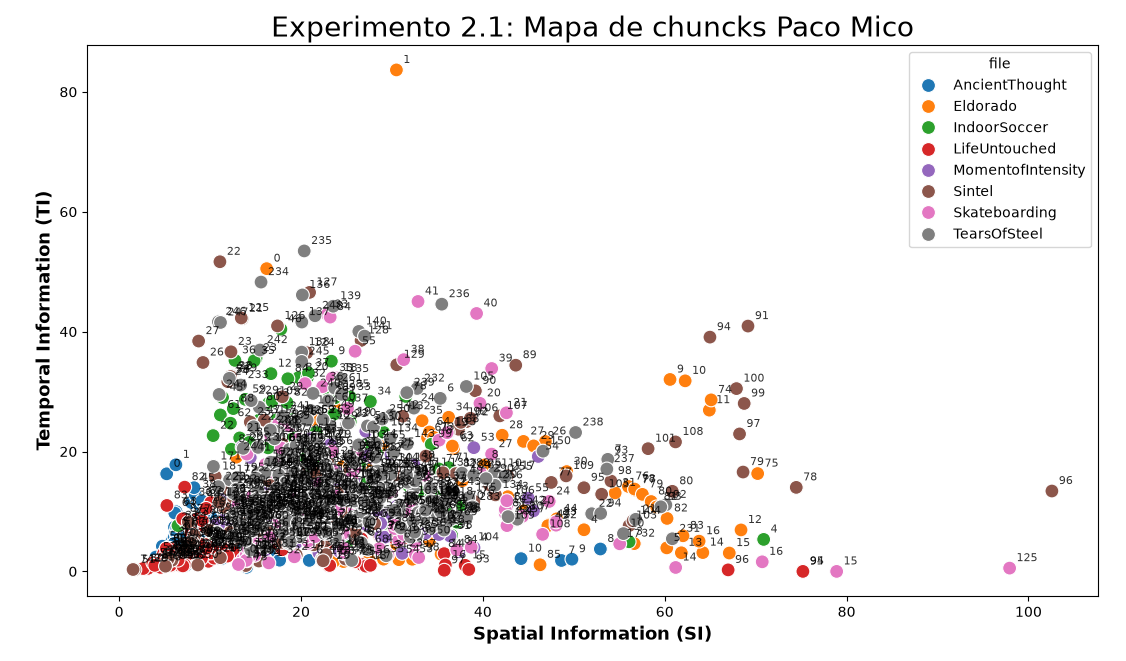
\includegraphics[width=\textwidth]{figs/exp2.1-siti-pacomico.png}
        \captionof{subfigure}{Ubicación de chunks de video en base a los datos del doctor Paco Mico}
        \label{fig:exp2.1-chunks-data-pacomico}
    \end{minipage}
     \hfill
     
    \begin{minipage}[b]{0.48\textwidth}
        \centering
        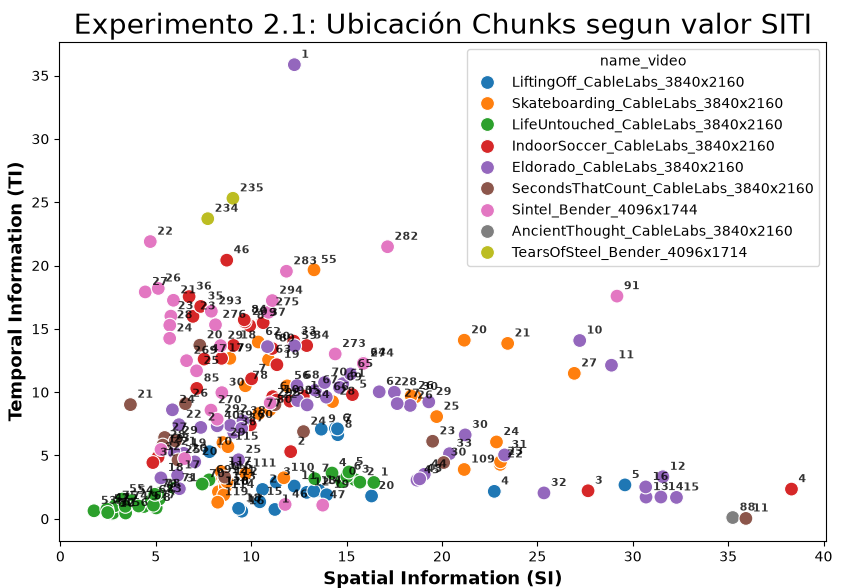
\includegraphics[width=\textwidth]{figs/exp2.1-ChucnkSITI-01.png}
        \captionof{subfigure}{Ubicación de chunks de video según el SI y el TI}
        \label{fig:exp2.1-chunks-selection}
    \end{minipage}
    
    \caption{Graficas que ubican la posicion de los chuncks en base a las metricas SI y TI}
    \label{fig:exp2.1-chunks-combined}
\end{figure}

Una vez determinada la posición de cada \textit{chunk} en función de sus valores de SI y TI, se definieron las cuatro zonas utilizadas para su clasificación, estableciendo para cada una de ellas los correspondientes rangos de SI y TI. El resultado de esta clasificación se recoge en la tabla \ref{tab:siti-zones-definition}.

Cabe destacar que la definición de los límites de cada zona presentó cierta dificultad, debido a que una gran parte de los chunks se concentra en la zona media-central del espacio SI-TI. Por este motivo, los rangos establecidos para las diferentes zonas presentan valores relativamente próximos entre sí. Asimismo, se encontraron dificultades para obtener chunks con valores elevados de TI, ya que no se identificó ningún \textit{chunk} con un valor superior a 35. De forma similar, los valores de SI obtenidos no superaron el valor de 45.


\begin{table}[h]
     \centering
     \begin{tabular}{|c|ccc}
     \cline{1-1}
     \rowcolor[HTML]{9B9B9B} 
     \textbf{Categoria} & \textbf{Etiqueta de Referencia} & \textbf{SI}                          & \textbf{TI}                         \\ \hline
     Bajo SI y Bajo TI  & \multicolumn{1}{c|}{LSI\_LTI}   & \multicolumn{1}{c|}{\textgreater 5}  & \multicolumn{1}{c|}{\textgreater 5} \\ \hline
     Alto SI y Bajo TI  & \multicolumn{1}{c|}{HSI\_LTI}   & \multicolumn{1}{c|}{\textless 25}    & \multicolumn{1}{c|}{\textgreater 5} \\ \hline
     Bajo SI y Alto TI  & \multicolumn{1}{c|}{LSI\_HTI}   & \multicolumn{1}{c|}{\textgreater 10} & \multicolumn{1}{c|}{\textless 16}   \\ \hline
     Alto SI y Alto TI  & \multicolumn{1}{c|}{HSI\_HTI}   & \multicolumn{1}{c|}{\textless 15}    & \multicolumn{1}{c|}{\textless 8}    \\ \hline
     \end{tabular}
     \label{tab:siti-zones-definition}
     \caption{Zonas de video para la clasificacion de chuncks en base al SITI}
\end{table}
 
\subsection{Consumo energetico en relacion al SITI}
% FASE 2.2 
 % - Videos para pruebas:
 %  - Seleccion de chuncks + necesidades de duracion de cada video
 %  - Creacion video continuo para descartar eficiencia intrinseca de los encoders
 %  - Figura de los chunks seleccionados
 % - Ejecucion de pruebas
 %    - Como se ejecutaran las pruebas
 %    - Script que lo ejecutara
 %    - Como y donde almacena los datos
 % - Pos procesameinto de los datos
 %    - Script de python que procesa datos
 %    - Como procesa y almacena datos en CSV
 %    - Grafica que genera
 % - Analisis de resultados
% SELECCION VIDEOS
En este primer subapartado se ha definido el conjunto de vídeos que se utilizará para analizar la relación entre el consumo energético asociado al proceso de codificación y los valores de las métricas \textbf{SI} y \textbf{TI}. Para ello, se requirieron vídeos de \textbf{10 segundos de duración} que no presentaran cambios de escena significativos ni cortes bruscos que pudieran alterar los valores medios de las métricas \textbf{SI} y \textbf{TI}. 

Para generar los vídeos utilizados en los experimentos se siguieron dos estrategias diferentes. La primera estrategia consistió en seleccionar un único \textit{chunk} y reproducirlo de forma continua hasta alcanzar una duración de 10 segundos, utilizando ffmpeg de la siguiente forma \lstinline[language=sh,label={code:ffmpeg-loopvideo},caption={}]{ffmpeg -y -stream_loop 15 -i CHUNCKXXX.mp4 -t 30 -b:v 30000k -r 30 -c:v copy -an VIDEO_10S_CHUNCKXXX.mp4}. De esta forma, se evitó introducir cambios bruscos de escena y se mantuvieron las características espaciales y temporales del \textit{chunk} original. Cada vídeo generado se identificó mediante el nombre del vídeo de procedencia y el número del \textit{chunk} seleccionado.

La segunda estrategia consistió en generar un vídeo a partir de la concatenación de la mayor cantidad posible de \textit{chunks} pertenecientes a una misma zona, utilizando además los \textit{chunks} consecutivos correspondientes al vídeo original. Esta estrategia permitió reducir la variabilidad que pudiera derivarse de las características internas de optimización de cada códec durante el proceso de codificación. Los vídeos generados mediante esta estrategia se identificaron utilizando el nombre del vídeo original y el identificador del primer \textit{chunk} empleado, correspondiente al \textit{chunk} \textit{0000}.

En total, se seleccionaron \textit{cinco vídeos por zona}, a excepcion de las zonas \textbf{HTI\_LSI}, habiendo añadido un video mas, y \textbf{HTI\_HSI}, habiendo añadido dos videos de mas. Adicionalmente, se ha generado un video por zona empleando varios chunks, lo que ha resultado en una muestra final de \textit{28 vídeos}. Resultanes se muestran en la tabla \ref{tab:exp2.2-videos}.

\begin{table}[h!]
 \centering
 \small   % Reducimos un poco el tamaño de letra
 \begin{tabularx}{\textwidth}{|>{\centering\arraybackslash}X|>{\centering\arraybackslash}X|>{\centering\arraybackslash}X|>{\centering\arraybackslash}X|}
 \hline
 \rowcolor[HTML]{C0C0C0}
 \textbf{LSI\_LTI} & \textbf{HSI\_LTI} & \textbf{LSI\_HTI} & \textbf{HSI\_HTI} \\
 \hline
 LifeUntouched\_0053                 & Sintel\_0021                         & Eldorado\_0014                & Skateboarding\_0027                 \\ \hline
 LifeUntouched\_0055                 & Sintel\_0026                         & Eldorado\_0016                & Skateboarding\_0021                 \\ \hline
 LifeUntouched\_0048                 & Sintel\_0027                         & Eldorado\_0012                & Skateboarding\_0020                 \\ \hline
 LifeUntouched\_0075                 & IndoorSoccer\_0046                   & Eldorado\_0015                & Eldorado\_0011                      \\ \hline
 LifeUntouched\_0056                 & Sintel\_0022                         & IndoorSoccer\_0004            & Eldorado\_0010                      \\ \hline
 LifeUntouched\_0000 {[} 51 - 55 {]} & TearsOfSteel\_0235                   & Eldorado\_0000 {[} 12 - 16{]} & Sintel\_0091                        \\ \hline
 \textbf{-}                          & TearsOfSteel\_0234                   & \textbf{-}                    & Skateboarding\_0000 {[} 20 - 25 {]} \\ \hline
 \textbf{-}                          & TearsOfSteel\_0000 {[} 231 - 235 {]} & \textbf{-}                    & \textbf{-}                          \\ \hline
 \end{tabularx}
 \caption{Videos creados para la experimentación de consumo energético en relación con las métricas SITI}
 \label{tab:exp2.2-videos}
\end{table}

% SELECCION DE EXPERIMENTOS
La fase de experimentacion se ha llevado a cabo empleando el script \textbf{exp2.2-sisti-energy} \ref{code:exp2.2-sitienergy}, desarrollado en bash. Este lleva a cabo la transcodificcion de cada uno de los videos \ref{tab:exp2.2-videos} empleando con cada uno de los codficadores especificados en \ref{tab:exp2-codecs-selection}, junto con los correspondientes bitrates definidos para cada generacion de codificadores. Adicionalmente, el script permite realizar todo el proceso de transcodificacion y toma de metricas son muliples contenedores simultaneamente. No obstante, en los experimentos realizados en esta fase se utilizó un único contenedor, sin establecer restricciones sobre el número de CPU y\/o núcleos disponibles.

El resultado de la toma de metricas de cada uno de los proceso de transcodificacion es almacenado en la estructura de directorios \ref{fig:exp2.2-datapath}, siendo el primero de todos el nombre del experimento. Esta estructura se diseñó con el objetivo de facilitar la automatización del procesamiento posterior de los datos mediante un script de Python.

\begin{figure}[h!]
    \centering
    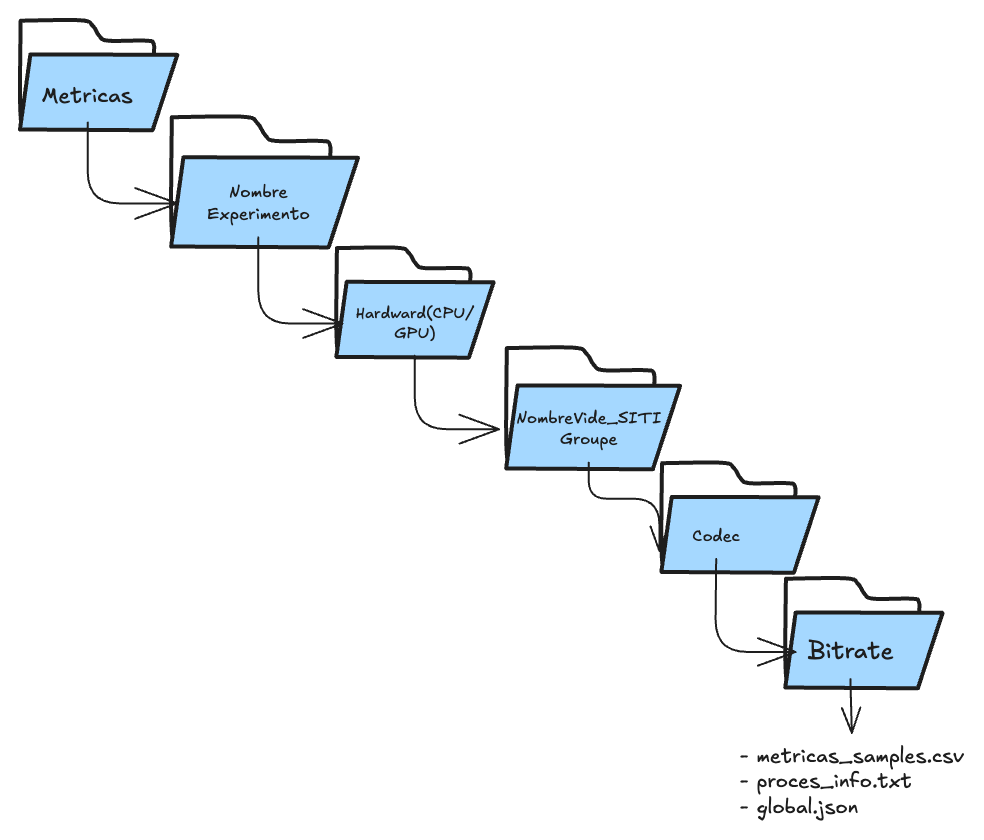
\includegraphics[width=0.45\linewidth]{figs/exp2.1-DataPathSITI.png}
    \caption{Estructura de directorios en la que se almacenan los datos de consumo de cada iteracion}
    \label{fig:exp2.2-datapath}
\end{figure}

%POST-PROCESAMIENTO DATOS
El postprocesamiento de las métricas recopiladas se realizó mediante el script de Python \textbf{ploter-exp2.2} \ref{code.2-ploter} \ref{code.2-ploter-obj}. Este script permite procesar y estructurar los datos obtenidos, almacenándolos en un archivo CSV con la estructura mostrada en \ref{fig.2-csvheader-dataprocess}. Asimismo, permite generar diferentes representaciones gráficas a partir de los datos procesados.

El script está diseñado para ejecutarse desde la interfaz de línea de comandos (\textit{CLI}), mediante diferentes \textit{flags} que permiten especificar tanto el tipo de procesamiento que se desea realizar como la ubicación de los datos de entrada. Las principales opciones disponibles son las siguientes:

\begin{itemize}
     \item \textbf{process}: permite procesar las métricas de consumo obtenidas durante el experimento \textit{exp2.2}. Por defecto, el script accede al directorio \textit{AllMetrics}, aunque es posible especificar una ruta alternativa.
     \item \textbf{plot3d}: permite representar la posición de cada vídeo en un gráfico tridimensional, en el que el eje X representa el valor de TI, el eje Y el valor de SI y el eje Z el consumo energético del contenedor. Se genera una gráfica para cada combinación de codificador y \textit{bitrate}.
     \item \textbf{plot-consumo-ti}: permite generar una gráfica bidimensional de tipo \textit{stream} para cada combinación de codificador y \textit{bitrate}. En este caso, el eje X representa el valor de TI y el eje Y el consumo energético, expresado en julios, del proceso de transcodificación.
     \item \textbf{plot-consumo-si}: permite generar una gráfica bidimensional de tipo \textit{stream} para cada combinación de codificador y \textit{bitrate}. En este caso, el eje X representa el valor de SI y el eje Y el consumo energético, expresado en julios, del proceso de transcodificación.
\end{itemize}

Por defecto, el script \textbf{ploter-exp2.2} determina el directorio en el que se almacenarán los datos resultantes del procesamiento, así como el directorio destinado al almacenamiento de las gráficas generadas. Asimismo, muestra los datos correspondientes al consumo energético de un único contenedor. No obstante, estos parámetros pueden modificarse mediante las siguientes opciones:

\begin{itemize}
     \item \textbf{--data-final-dir=PATH\_ARCHIVO}: permite definir una ruta alternativa para almacenar el archivo CSV resultante del procesamiento de los datos. Por defecto, se utiliza la ruta \textit{./data/ex2.2\_process\_data.csv}.
     \item \textbf{--container=consumo\_container0\_j}: permite seleccionar el contenedor cuyos datos de consumo se utilizarán para generar las gráficas, en caso de que se hayan ejecutado varios contenedores. Por defecto, se utilizan los datos correspondientes a la columna \textit{consumo\_container0\_j}.
\end{itemize}

% ANALISI DE RESULTADOS
% % RESULTADOS:
%   - El consumo energetico se ve afectado severamente por el numer de FPS de cada video, ay que al codificar el mismo video con diferentes FPS se obtiene un consumo mucho mayor a mayor cantidad de FPS.
% - Timpos de los video demasiado bajos para apreciar diferencias en la codificacion con tarjeta grafica
% - Se requiere mayor diversidad de videos con valores todavia mas altos de SI y TI
% - Se observa que hay otro tipo de metricas subjetivas que afectan al consumo energetico mas halla del SITI
%   - Para x264:
%        - El TI influye en el consumo energetico
%   - Para x265:
%        - El Ti influye pero no es del todo concluyente
%   
%   - Para H264:
%        - Las metricas de consumo son muy similares pero se puede observar que el SI es quien mas influye en el consumo energeticp 
%    - Para H265:
%        - Influye SI y Ti en consumo pero no se puede establecer correlacion clara, metricas de consumo muy similares


% AMPLIACION 1:
%    - Para descartar la eficiencia de los codificadores a la hora de codificar video y predecir la siguiente trama, se han creado una total de 4 videos empleando los chuncks de la sigiuente list \ref{list:chubkc-videos-fase2.2}, ubicando cada uno de estos videos en una de las zonas establecidas en base al SITI. 
%    - Como resultado xxxx

El conjunto de graficas obtenidas mediante el script de Python \textbf{ploter-exp2.2} a partir de las metricas resultantes del proceso experimental, llevado a a cabo por el script en Bash \textbf{exp2.2-sisti-energy}, unicamente se mostrar algunas de ellas para facilitar el analisis y el resto se se encuentran al completo en el apendice RRR ReF. Esto se debe a que hay un gran numero de graficas e insertarlar todas en este apartado incomodaría al lector.

\tresubfigs
     {figs/exp2.2/ploter2.2/plot3d/consumo_container0_j-libx264-30_ConsumoSITI.png}{Consumo energetico frente a Si y TI codificado con libx264 a 30 Mbps}{fig:exp2.2-plot3d-libx264-30}
     {figs/exp2.2/ploter2.2/consumo-si/consumo_container0_j-libx264-30_ConsumoSI.png}{Consumo energetico frente a SI codificado con libx264 a 30 Mbps}{fig:exp2.2-consumoxti-libx264-30}
     {figs/exp2.2/ploter2.2/consumo-ti/consumo_container0_j-libx264-30_ConsumoTI.png}{Consumo energetico frente a TI codificado con libx264 a 30 Mbps}{fig:exp2.2-consumoxsi-libx264-30}

 

\subsection{Relación entre numero de cores, tiempo de codificación y consumo energetico}
% - EXPERIMENTACION THREADS CONSUMO
%    - Se espera comprobar si el numero de threads empleando en el proceso de codificacion influye en el tiempo de codificacion y en el consumo energetico
%    - DataSet de videos
%         - Seleccion de dos vidos por zona, lo que da un total de 8 videos + 4 videos formados por videos de chincks consecutivos
%         - Duracion de 30 segundos cada video
%         - 30 frames 
%         - 4k
%         - Lista de chuncks seleccionados \ref{lst:chuncks}
%    - Se ha modificado script de anterior subfase experimental para que:
%         + Itere sobre contenedores con limited en numero de cores y cpus[1,3,6,7,ningun]
%         + Se llevar a cabo el proceso de codificacion selectivo dependiendo de el numero de cpu que disponga el contenedor \ref{tabla_workflows} (Explicar Funcionamiento de cada Codificador y limitaciones en indicar numero de threads en cada uno)
%         + Se lleva a cabo codificacion con 10 Mbps y a 30 Mbps, ya que a el Bitrate influye en el consumo energetico y se quiere como afecta a resultados finales
%         + No se lanzan contenedores en paralelo pero script soporta definicion multiples contenedores para ampliaciones futuras
%    - procesameinto de datos con script ploter-2.3
%         - Como procesa y almacena datos en CSV + Estructura
%         - Graficas que genera
%    - Analisis de graficas 
%    -Conclusiones Subfase 2 experimentacion
%         

% EXP 2.3 --> Fase en la que se limita el numero de cores en el contenedor y se fueza el mismo numero de threads para ffmpeg
%   + CORES = {0,1,3,6, 7}, donde 0 hace referencia a ninguna limitacion de cpu y de threads
%   + THREADS = CORES

 % FASE 3.0: VIDEOS A UTILIZAR - **SUJETO A CAMBIOS**
 % - Para esta fase se utilizran 8 videos, uno por cada zona designada en base al SI y al TI \ref{lst:lista-zonas-exp2}, los cuales tendran una duracion de 30 segundos. La trascodificacion se llevara a cabo para con un bitrate de bajo requerimiento, como es 10 Mbps, y un bitrate con mayor requerimiento, siendo en este caso 30 Mbps. 
 % - Los codecs a utlizar seran los mismo que se han testado en la segunda fase de experimentacion, subseccion 2 \ref{exp2.2-codec-bitrate}. 
 % - En cuanto al bitrate se ha definido como valor constante 30 Mbps como valor constante para los cuatro condificadores x264, H264_NVENC, x265 y HEVC_NVENC. Ya que no existen mejoras de calidad perceptibles con btr superiores pero si se percibe el cambio respecto a btr inferiores. 
 % - Los chuncks que formaran parte de esta seccion son: 
 %   -  HT_LSI: 
 %        - TearOfSteel_0235
 %        - Sintel_0027
 %   -  HTI_HSI
 %        - El Dorado_0010
 %        - Skate_0020
 %   -  LTI_HSI
 %        - IndorSoccer_0004
 %        - ElDorado_0015
 %   -  LTI_LSI
 %        - LifUntouch_0053 
 %        - LifUntouch_0056
 %- La codificacion se llevara a cabo video a video, minimizando el numero de tareas del sistem.


 % Fase 3.1: SELECCION DE UNA CONFIGURACION DE FFMPEG 
 % - Se debe de seleccionar una configuracion para cada codec, que permita delimitar el numero de threads que es capaz de utilizar al transcodificar
 % - Configuracion de ffmpeg para utilizar threads y cores, obtener configuraciones disponibles para cada codec con *ffmpeg -h long encoder=CODEC_NAME*
 %   -libx264:
 %        - Orden --> ffmpeg -y -i VIDEO_ENTRADA -c:v libx264 -threads X -thread_type frames -b:v 30M -c:a copy RUTA_VIDEO_FINAL
 %        - Informacion sacada de FFMPEG Wiki y de PAPER THREADS 
 %        - Prueba de funcionamiento IMG-exp3.2-libx264-threads
 %   -libx265:
 %        - Orden --> ffmpeg -y -i VIDEO_ENTRADA -c:v libx265 -x265-params frame-threads=X:pools=X -b:v 30M -c:a copy RUTA_VIDEO_FINA
 %        - Informacion sacada de FFMPEG 265 WIKIy de PAPER THREADS 
 %        - Prueba de funcionamiento IMG-exp3.2-libx265-threads
 %   -H264: 
 %        - Orden --> ffmpeg -y -i VIDEO_ENTRADA -c:v h264_nvenc -cpucount X_cpus  -b:v 30M -c:a copy RUTA_VIDEO_FINAL
 %        - Se limita numero de CPUs que puede utilizar el codificador, informacion encontrada mediante 'ffmpeg -h encoder=h264_nvenc'
 %   -HEVC:
 %        - Orden --> ffmpeg -y -i VIDEO_ENTRADA -c:v h264_nvenc -cpucount X_cpus  -b:v 30M -c:a copy RUTA_VIDEO_FINAL
 %        - Se limita numero de CPUs que puede utilizar el codificador, informacion encontrada mediante 'ffmpeg -h encoder=h264_nvenc'
 % Script del experimento 2.3:
 % - Se ha empleado un script similar al de la fase 2.2 aplicando modificaciones:
 %   - Arranque de contenedores de forma dinamica con limitacion en el numero de CPUs
 %   - Limitacion en numero de threads en la orden de ffmpeg para cada codficador
 % 
 % CONCLUSIONES:
 % - En el caso de cada codificador se han llegado a conclusiones interesantes:
 %   - X264:
 %        + Es bastante eficiente empleando threads pero si se observa que una cierta saturacion al alcanzar  numero de cores del sistema mas elevados, pareciendo que satura sobre los 7 - 8 cores
 %        + La diferencia de bit rate afecta a la cantidad de energia que se emplea en cada fase de codificacion, asi como en los tiemps que esta requiere. A mayor es el bitrate mas intensa es la tarea de codificacion y mas visible se hace el intento de saturacion del que se ha hablado con anterioridad
 %   - x265:
 %        + Se observa que el codec se ajusta a la cantidad de cores y threads establecidos, consumiendo mayor cantidad de recursos en relacion al numero de cores y reduciendo el tiempo de codificacion.
 %        + Se puede on¡bservar cierta saturacin tanto con 10 como con 30 Mbps en el numero de cores aunque no se puede asegurara al 100 x 100, tambien se obsevan diferentes respuesta para cada video, en relacion a los valores SITI, aunque se sospecha que otras metricas pueden estar influyendo.
 %   - H264 y Hevc_nvenc:
 %        + Se observa saturacion al rededor de los 6 cores, tanto para 10 como para 30 Mbps
 %        + El unico escenario en el que la eficiencia energetica es mejor es cuando no se limitan el numero de cores, aunque las metricas se encuentran muy cercanas a las obtenidas con 6 cores y 6 threads. 
 %        + Destacar que hevc_nvenc es un poco mas eficiente energeticamente respecto a h264
 %        + Tambien se debe destacar que al igual que en el resto de codecs, dependiendo del video se ven mejores performace en la codificacion, lo que indica que tanto el SITI como otras metricas del video estan afectando al consumo y a los tiempos del proceso de codificacion. 
 %    
 % - Si se observan las graficas de consumo de los codecs que funcionan unicamente sobre CPU frente a los que emplean GPU+CPU, se puede aprecias que aquellos que utilizan codificacion basada en GPU consumen mucho menos recursos energeticos y necesitan de un menor tiempo para llevar a cabo el proceso. 
 % - 
 % - Se debe tener en cuenta el entorno en el que se han desarrollado las pruebas cuenta unicamente con 8 cores, lo cual no nos ha permitido encontrar el limite en el numero de cores y establer un numero que sature la utilidad de threads con firmeza para cada encoder
 % 